\section{Method}

\setLayout{mainpoint}

\begin{frame}[noframenumbering, plain]{}
    \frametitle{Method}
\end{frame}

\setLayout{blank}

%---------------------------------------------------------
\begin{frame}{Overview}
    \begin{figure}[!htb]
    \centering
        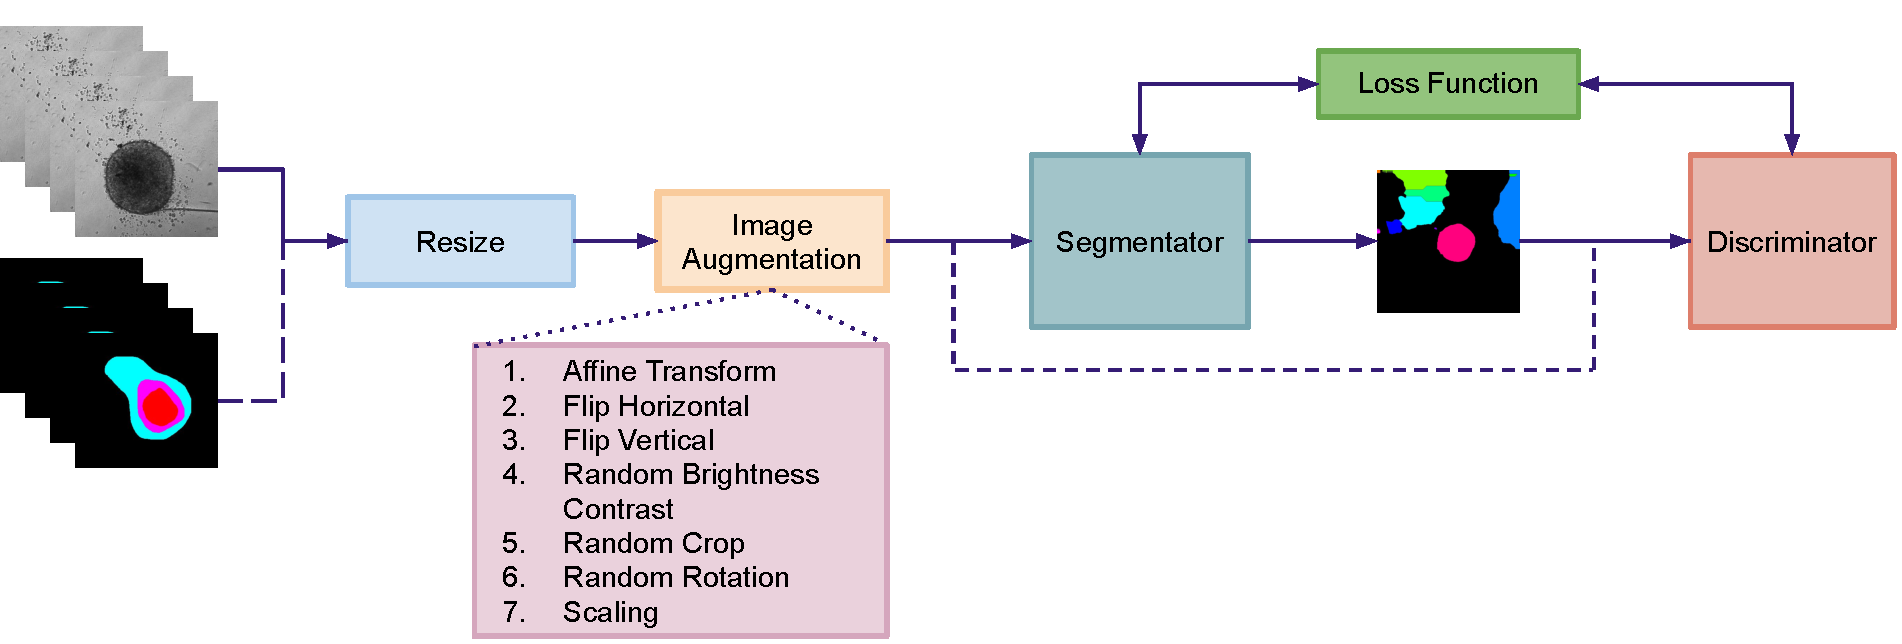
\includegraphics[width=15cm]{figures/method/overview}
        \label{fig:method_overview}
    \end{figure}
\end{frame}

%---------------------------------------------------------
\setLayout{horizontal}

\begin{frame}{Data Augmentation}
    \begin{figure}
        \centering
        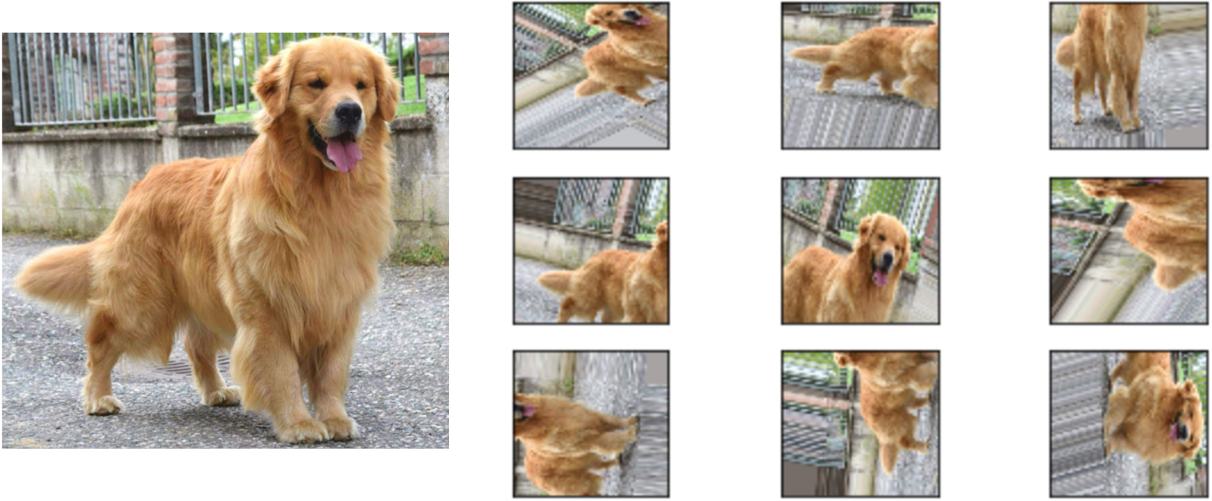
\includegraphics[width=13cm]{figures/method/data_augmentation}
    \end{figure}
\end{frame}

%---------------------------------------------------------
\setLayout{blank}

\begin{frame}{Generator Architecture}
    \begin{figure}[!htb]
        \centering
        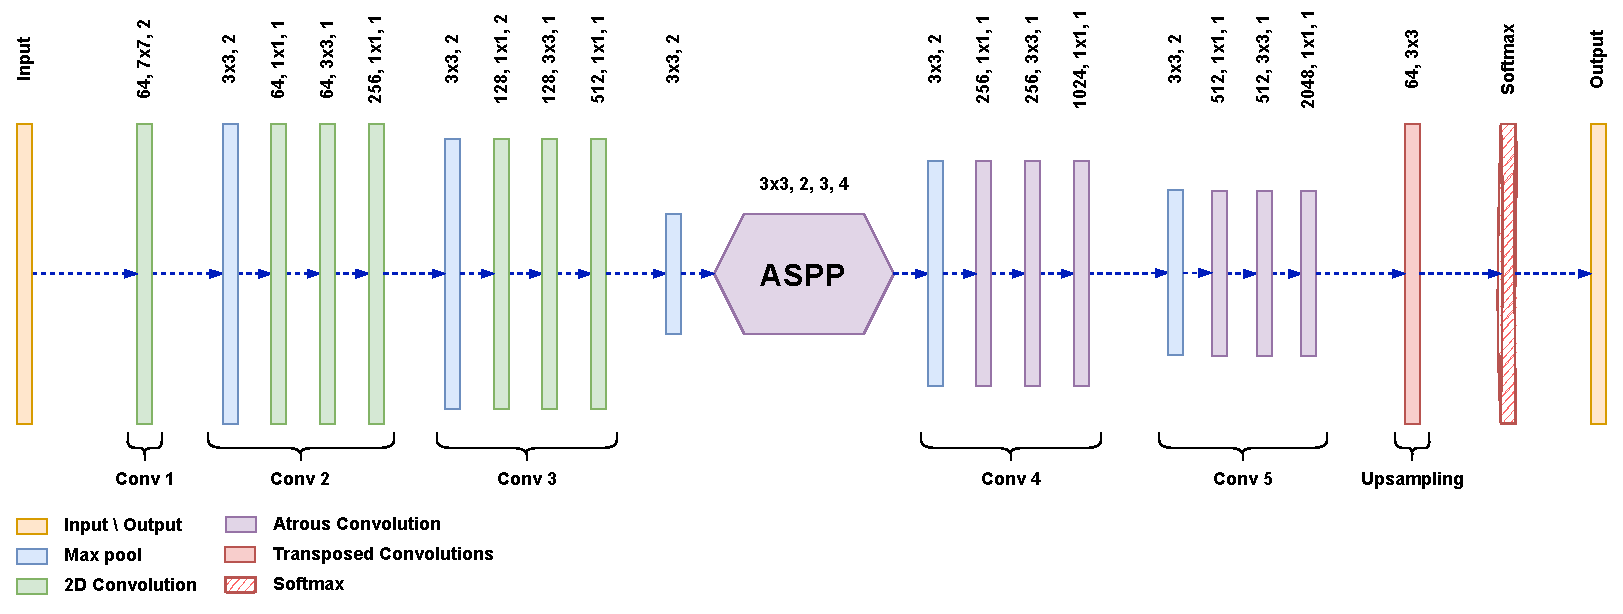
\includegraphics[width=14cm]{figures/method/generator_architecture}
    \end{figure}
\end{frame}

%---------------------------------------------------------

\begin{frame}{Discriminator Architecture}
    \begin{figure}[!htb]
        \centering
        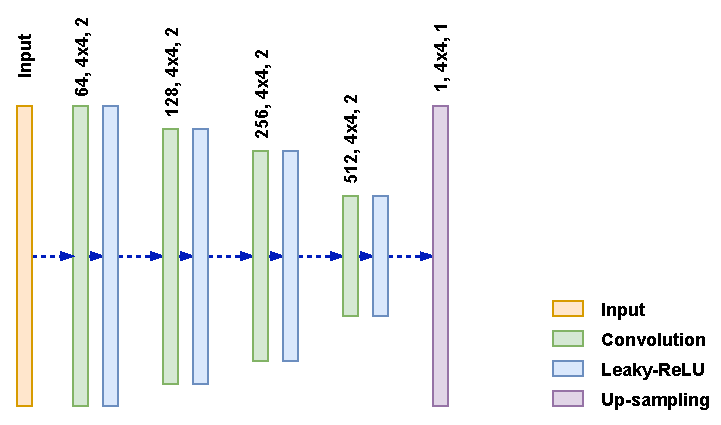
\includegraphics[width=10cm]{figures/method/discriminator_architecture}
    \end{figure}
\end{frame}

%---------------------------------------------------------
\setLayout{vertical}

\begin{frame}{Loss Functions}
    \begin{block}{Generator Loss}
        \begin{equation}
            \label{eq:seg_loss}
            \mathcal{L}_{seg} = \mathcal{L}_{ce} + \lambda_{adv}\mathcal{L}_{adv} + \lambda_{semi}\mathcal{L}_{semi}
        \end{equation}
    \end{block}
\end{frame}

%---------------------------------------------------------
\begin{frame}{Evaluation Metrics}
    \begin{columns}
        \column{0.5\textwidth}
        Dice Coefficient
        \begin{figure}[!htb]
            \centering
            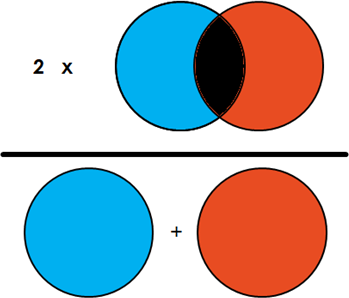
\includegraphics[width=5cm]{figures/method/dice_coefficient}
        \end{figure}
        \column{0.5\textwidth}
        Jaccard Index
        \begin{figure}[!htb]
            \centering
            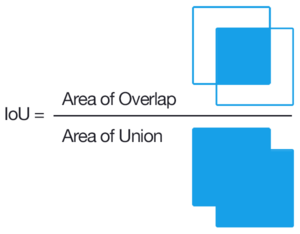
\includegraphics[width=5cm]{figures/method/jaccard_index}
        \end{figure}
    \end{columns}
\end{frame}

%---------------------------------------------------------
\setLayout{horizontal}

\begin{frame}{Watershed}
    \begin{figure}
        \centering
        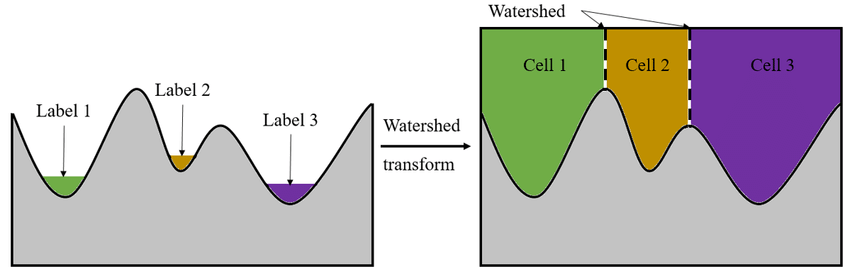
\includegraphics[width=15cm]{figures/method/watershed}
    \end{figure}
\end{frame}
